\section{Compiler Overview}
Figure \ref{Fig:CompilerStructure} shows the high level structure of Treebeard. 
The input to TreeBeard is a JSON serialized decision forest model, it supports popular frameworks like XGBoost and LightGBM and is extensible to other frameworks.
Given an input model our compiler generates optimized inference code. Specifically it generates a callable batch inference function \texttt{predictForest} that given an array of inputs, outputs an array of model predictions. 
 
TreeBeard specializes the code generated for inference by progressively optimizing and lowering a high level representation of the \texttt{predictForest} function down to LLVM IR \cite{LLVM}.
It is implemented as a dialect in the MLIR framework \cite{MLIR},
%Treebeard first constructs a high level representation of the decision forest inference operation. 
 At this level (HIR) it applies transformations that determine how inputs traverse the decision forest. It re-order trees in the forest and determines the high level loop structure (process one tree at a time or one input at a time). It then lowers to a traditional loop based IR (MIR). Several loop level optimizations like unrolling and pipelining are applied at this level. At the lowest level of IR TreeBeard applies layout optimizations and generates parallel code in LLVM IR. 
LLVM is then used to JIT compile the generated IR to executable code. The following sections describe each level of the IR and their lowering in more detail.

 %The specified set of options includes information such as the batch size, the type of the input features, the type for node thresholds and the type for feature indices \TODO{There are also several optimization related inputs like tile size, type of tiling, pipeline depth etc. Should we mention those?}. 


\begin{figure}
  \centering
  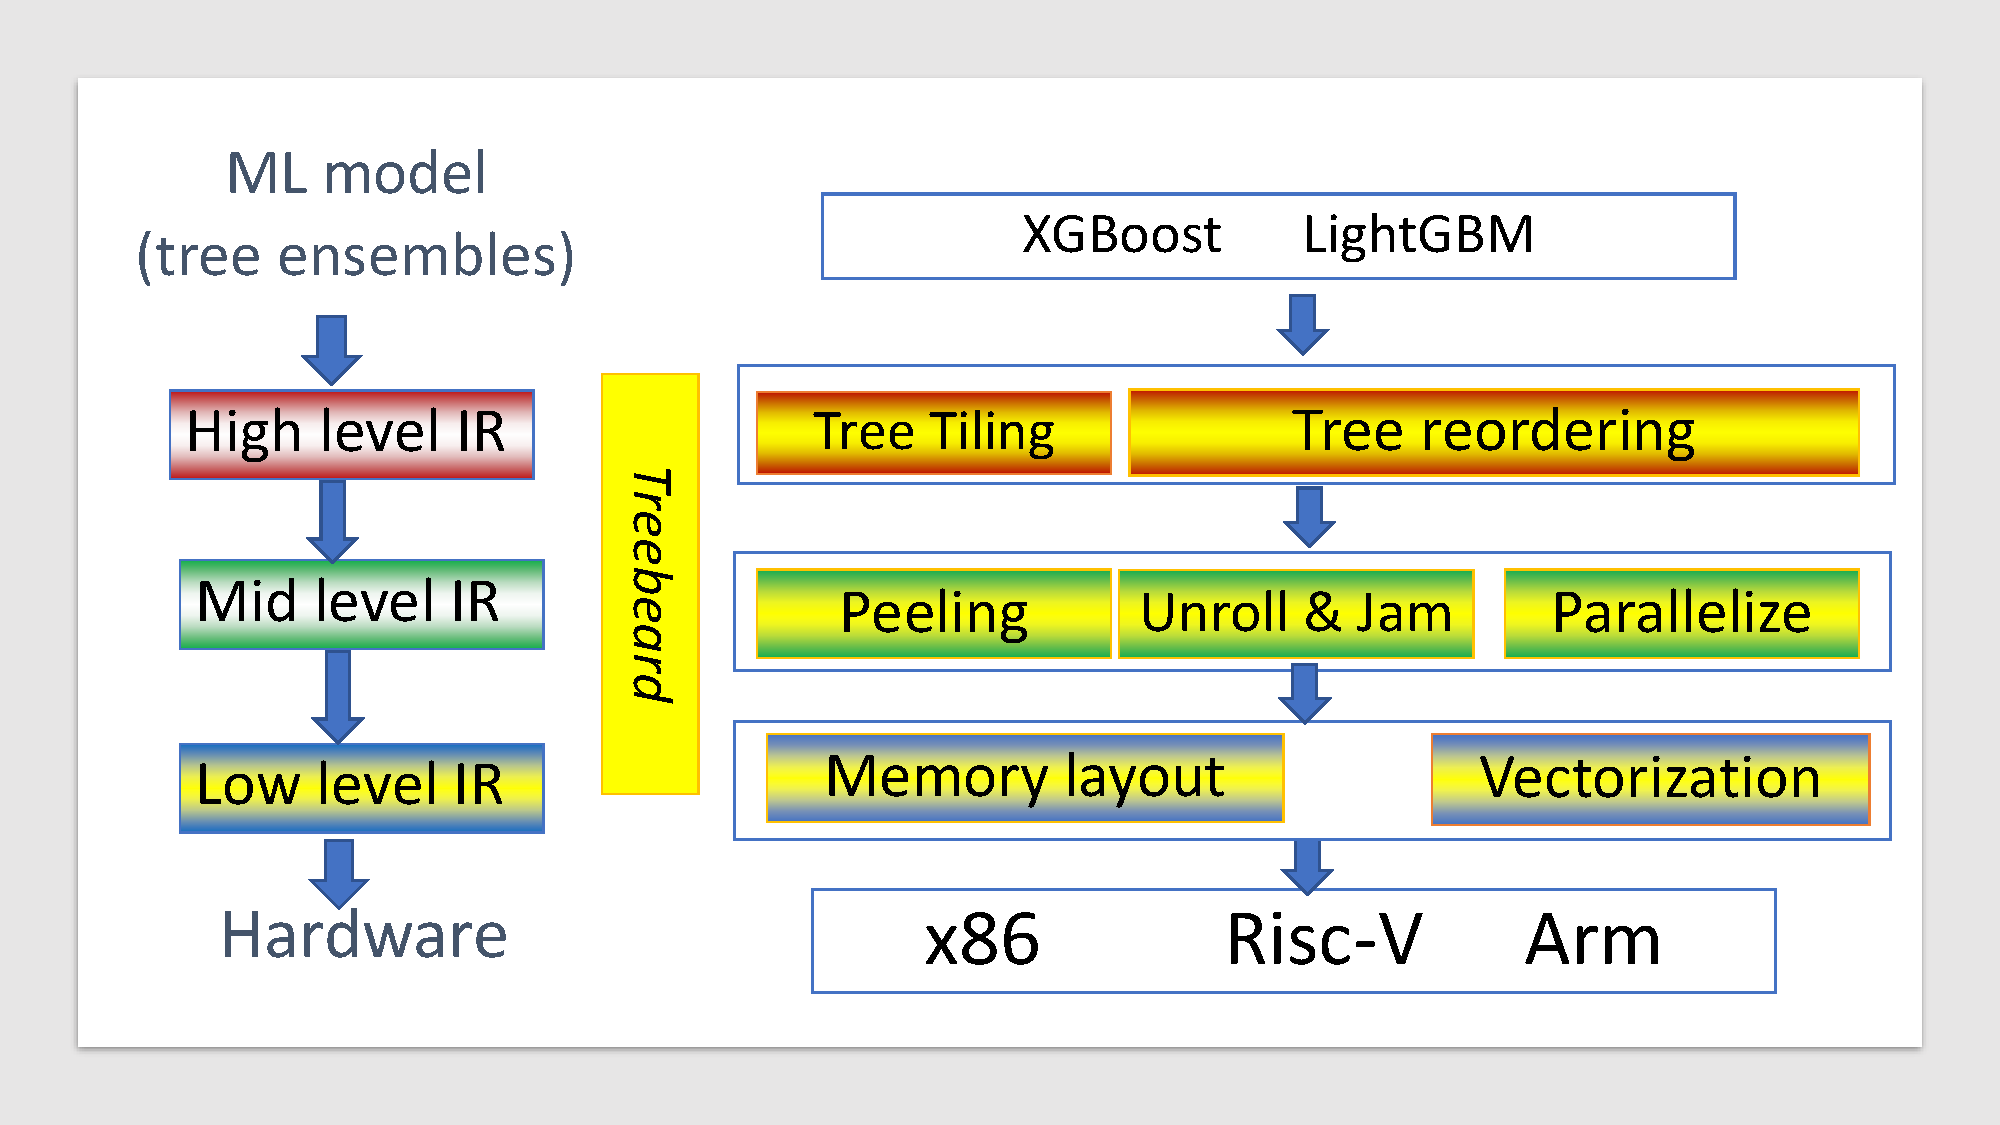
\includegraphics[width=\linewidth]{figures/compiler.pdf}
  \caption{Treebeard Compiler Structure}
  \label{Fig:CompilerStructure}
\end{figure}

\TODO{Should we describe the dialect's type system?}
\TODO{Kr : consider focusing on the example instead of verbose description of optimizations. This section can be short, descriptions can come in later sections.}
\subsection{High Level IR}
Treebeard parses the input JSON file and generates a function with a single MLIR operation, \texttt{predictForest} that represents inference using the input model on a set of rows. The operation contains within it a tree based representation of the model that can be manipulated by optimizing transformations. Transformations on the model such as tiling, tree reordering and leaf padding are done at this level. The structure of the loop nest to walk the iteration space of trees and inputs is also decided at this level of the IR. \TODO{Should we mention that there is a scheduling language to decide this?}

\begin{lstlisting}[language=C++]
func Predict(float rows[batchSize]) {
  predictions = predictForest(rows) 
  return rows
}
\end{lstlisting}

\subsection{Mid Level IR}
The Mid Level IR makes the loop structures and tree walks more explicit. Firstly, the order in which the iteration space of trees and inputs is walked is explicitly specified in the IR through loop nests. Also, tree specific operations such as \texttt{isLeaf}, \texttt{traverseTile}, \texttt{getLeafValue} are introduced so that the traversal of trees explicitly represented. The following listing shows the IR for inference using a model with four trees on an input batch with two rows. The listed IR walks all trees for one input row before moving to the next row. One important point to note here is that details such as the data structure used for the trees are not explicitly encoded in the IR. This allows us to reuse optimization and lowering passes on this level of the IR regardless of what the final in memory representation of the model is.

\begin{lstlisting}[language=C++]
  // Constant that represents the model being compiled
  forest = ensemble(...)
  for i = 0 to 2 step 1 {
    prediction = 0
    for t = 0 to 4 step 1 {
      tree = getTree(forest, t) 
      node = getRoot(tree)
      while (isLeaf(tree, n)==false)  do {
        node = traverseTreeTile(tree, node, rows[i])
      }
      treePrediction = getLeafValue(tree, node)
      prediction = prediction + treePrediction
    }
    predictions[i] = prediction
  }
\end{lstlisting}

The IR listed above is a simplification of the actual IR. The actual IR is strongly typed and in SSA form.

\subsection{Low Level IR}
The IR is finally lowered to a form where the in memory representation of the model is made explicit. Buffers to hold the model values are inserted into the generated code and all tree operations in the mid-level IR are lowered to explicitly reference these buffers. The semantics of all operations are made explicit. For example, \texttt{traverseTreeTile} is lowered into a series of operations to load thresholds, feature indices and features, compare the features with the thresholds and compute the next node to evaluate. This IR is then lowered directly to LLVM IR and JITted.

